\documentclass[aspectratio=1610,10pt]{beamer}
%\usepackage{titlesec}

%\usepackage{setspace}
%\linespread{1.2}
\setlength{\parskip}{4pt}
%\usepackage{indentfirst}
%\usepackage[margin={1.5in, 1.5in}]{geometry}
%\usepackage[bottom]{footmisc}

\usepackage[dvipsnames]{xcolor}
\def\TEXTCOLOR {black}
\def\PAGECOLOR {white}
\def\NOTECOLOR {Purple}
\definecolor{linkBlue}{rgb}{0,.25,.55}

\color{\TEXTCOLOR}
\pagecolor{\PAGECOLOR}

% \titleformat{\part}[hang]{\Large\bfseries\filcenter}{\thepart}{1em}{}
%\titleformat{\section}[hang]{\large\bfseries\filcenter}{\thesection}{1em}{}
%\titleformat{\subsection}[hang]{\bfseries}{\thesubsection}{1em}{}

\usepackage{amsmath}
\usepackage{amssymb}
\usepackage{bbm}
\usepackage{mathtools}
\usepackage{amsfonts}
\usepackage{comment}
%\usepackage{ulem}
%\usepackage{enumitem}
\usepackage[mathscr]{euscript}
\usepackage{tikz-cd}
%\usepackage{slashbox}
\usepackage[margin=1in]{caption}

\usepackage{mathrsfs}
\usepackage{appendix}
\usepackage[backend=biber,style=alphabetic,maxnames=5,maxcitenames=5,sorting=ynt]{biblatex}
\usepackage{wrapfig}

%\usepackage[pdftex, psdextra]{hyperref}
% \hypersetup{
% 	colorlinks=true,
% 	linkcolor=linkBlue,
% 	filecolor=magenta,
% 	urlcolor=linkBlue,
% 	citecolor=linkBlue}
% \usepackage[nameinlink,noabbrev]{cleveref}

\usepackage{graphicx}
\graphicspath{{Images/}}
\usepackage{caption}
\usepackage{pgfplots}
\pgfplotsset{compat=1.18}

\newenvironment{todo}{\color{\NOTECOLOR}\begin{list}{$\Box$}{}}{\end{list}\color{\TEXTCOLOR}}

\usepackage{amsthm}
\theoremstyle{definition}
\begin{comment}
\newtheorem{definition}{Definition}[subsection]
\newtheorem{theorem}[definition]{Theorem}
\newtheorem*{theorem*}{Theorem}
\newtheorem{corollary}[definition]{Corollary}
\newtheorem{lemma}[definition]{Lemma}
\newtheorem*{lemma*}{Lemma}
\newtheorem{proposition}[definition]{Proposition}
\newtheorem{remark}[definition]{Remark}
\newtheorem{example}{Example}[subsection]
\newtheorem*{example*}{Example}
\newtheorem*{definition*}{Definition}
\end{comment}
\newtheoremstyle{named}{}{}{\itshape}{}{\bfseries}{.}{.5em}{\thmnote{#3}}
\theoremstyle{named}
\newtheorem*{namedtheorem}{Theorem}

\let\emptyset\varnothing
\let\tilde\widetilde
\renewcommand{\bar}[1]{\overline{\hspace{-1pt}{#1}\hspace{-.2pt}}}
\let\hat\widehat
\newcommand{\de}{\text{d}}
%\newcommand{\del}{\partial}
%\newcommand{\delbar}{{\bar\partial}}
\newcommand{\eq}[1]{\begin{align*}{#1}\end{align*}}
\newcommand{\inlinetodo}[1]{\color{\NOTECOLOR} $\,\Box$ {#1}\color{\TEXTCOLOR}}
%\newcommand{\note}[1]{\color{\NOTECOLOR}{[{#1}]}\color{\TEXTCOLOR}}
\newcommand{\AY}[1]{{\color{violet}{\rm [AY: #1]}}}
\newcommand{\R}{\mathbb{R}}
\newcommand{\Q}{\mathbb{Q}}
\newcommand{\C}{\mathbb{C}}
\newcommand{\N}{\mathbb{N}}
\newcommand{\Z}{\mathbb{Z}}
\newcommand{\F}{\mathbb{F}}
\newcommand{\A}{\mathbb{A}}
\renewcommand{\P}{\mathbb{P}}
\renewcommand{\k}{\mathbbm k}
\renewcommand{\a}{\mathfrak a}
\newcommand{\ya}{\reflectbox{$\mathsf R$}}
\newcommand{\from}{\,:\,}
\newcommand{\into}{\hookrightarrow}
\newcommand{\onto}{\twoheadrightarrow}
\newcommand{\acts}{\mathbin{{\text{\raisebox{.75em}{\rotatebox{-90}{$\circlearrowright$}}}}}}
\newcommand{\horz}{\raisebox{-1pt}{\large\textbf{---}}}
\newcommand{\quot}[2]{\raisebox{1pt}{${#1}$}\big/\raisebox{-1pt}{${#2}$}}
\newcommand{\im}{\text{im}\,}
\newcommand{\sm}{\smallsetminus}
\newcommand{\eps}{\varepsilon}
\newcommand{\spec}{\text{Spec}\,}

%\DeclareMathOperator{\de}{\text{d}}
\DeclareMathOperator{\delbar}{\bar\partial}
\DeclareMathOperator{\del}{\partial}
\DeclareMathOperator{\tr}{tr}
\DeclareMathOperator{\rk}{rk}
\DeclareMathOperator{\diag}{diag}
\DeclareMathOperator{\GL}{GL}
\DeclareMathOperator{\SL}{SL}
\DeclareMathOperator{\U}{U}
\DeclareMathOperator{\SU}{SU}
\DeclareMathOperator{\SO}{SO}
\DeclareMathOperator{\Hom}{Hom}
\DeclareMathOperator{\End}{End}
\DeclareMathOperator{\Rep}{Rep}
\DeclareMathOperator*{\twoslash}{\hspace{-.2em}/\hspace{-.2em}/\hspace{-.2em}}
\DeclareMathOperator*{\fourslash}{\twoslash\twoslash}
\addbibresource{Main.bib}
\newcommand{\bx}{\mathbf{x}}
\newcommand{\by}{\mathbf{y}}

\usetikzlibrary{decorations.pathreplacing}


\title{Metric Convergence from Parabolic Higgs Bundle Moduli Spaces to Hyperpolygon Spaces}
\institute{University of Oregon}
\author{Arya Yae}
\date[June 19, 2026]{June 19, 2026 \\ \vspace{3ex} \small{Joint work with Laura Fredrickson}}

\begin{document}
\setbeamertemplate{itemize items}[circle]
%Taken from https://tex.stackexchange.com/questions/348/how-to-draw-a-torus
\tikzset{
  pics/torus/.style n args={3}{
    code = {
      \providecolor{pgffillcolor}{rgb}{1,1,1}
      \begin{scope}[
          yscale=cos(#3),
          outer torus/.style = {draw,line width/.expanded={\the\dimexpr6\pgflinewidth+#2*2},line join=round},
          inner torus/.style = {draw=pgffillcolor,line width={#2*2}}
        ]
        \draw[outer torus] circle(#1);\draw[inner torus] circle(#1);
        \draw[outer torus] (180:#1) arc (180:360:#1);\draw[inner torus,line cap=round] (180:#1) arc (180:360:#1);
      \end{scope}
    }
  }
}
\tikzset{
  pics/opentorus/.style n args={3}{
    code = {
      \providecolor{pgffillcolor}{rgb}{1,1,1}
      \begin{scope}[
          xscale=cos(#3)
        ]
        \begin{axis}[axis x line = none, axis y line = none, width = 24cm, height = 16cm, at = {(-5.2cm,-5.3cm)}]
            \addplot[black, line width = 3pt]{x^2};
        \end{axis}
        \draw[line width = 1pt] (6.8,-1.5) arc (270:90:2);
        \draw[line width = 1pt] (5.7,-1.1) arc (-90:90:1.6);
    \end{scope}
    }
  }
}

\frame{\titlepage}

%\newgeometry{left=.5in,right=.5in}
\begin{frame}
\tableofcontents
\end{frame}

\section{Preliminaries}
\subsection{Hyperkähler Manifolds}
\begin{frame}
    \frametitle{Hyperkähler Manifolds}
    \begin{definition}
            A \emph{hyperkähler} manifold is a $4n$-dimensional manifold with a triple of kähler structures $(X,g,I,J,K,\omega_I,\omega_J,\omega_K)$ such that $I,J,K$ satisfy the quaternionic relations.
    \end{definition}
    \vfill
    \pause

    Equivalently, $(X,g)$ has holonomy contained in $\text{Sp}(n)=\text{Sp}(n,\C)\cap \SU(2n)$.  In particular, $X$ is Ricci-flat.
    \vfill
    \pause

    The hyperkähler condition is very rigid.  The compact hyperkähler 4-manifolds are:
    \begin{itemize}
        \item Compact tori $\C^2/\Gamma$ for a lattice $\Gamma\cong\Z^4$
        \item K3 surfaces (simply connected)
    \end{itemize}
    \vfill
\end{frame}

\subsection{Recipe for Constructing Hyperkähler Manifolds}
\begin{frame}
    \frametitle{Recipe for Constructing Hyperkähler Manifolds}
    Any complex vector space has a natural kähler structure $(V,I,g,\omega)$ arising from the dot product and multiplication by $i$.
    \vfill
    \pause
    The cotangent bundle $X=T^*V$ of a complex vector space additionally has a holomorphic/algebraic symplectic form
        $$\Omega((u_1,w_1),(u_2,w_2))=w_1u_2-w_2u_1.$$
    Along with the standard kähler structure on $X$, we get a hyperkähler structure by decomposing $\Omega=\omega_J+i\omega_K$.
\end{frame}

\begin{frame}[t]
    \frametitle{Recipe for Constructing Hyperkähler Manifolds}
    Suppose $G\subset G_\C$ act on a hyperkähler space $(X,I,\omega,\Omega)$, respectively preserving $\omega$ and $\Omega$.
    \vfill
    \pause
    Suppose further the action admits moment maps $\mu_\R\from X\to\mathfrak g^*$ and $\mu_\C\from X\to\mathfrak g_\C^*$.  Given elements $\beta\in Z(\mathfrak g^*)$, $\tau\in Z(\mathfrak g_\C^*)$, one constructs the \emph{hyperkähler quotient} $X\underset{(\beta,\tau)}\fourslash G$ in two ways:
    \vfill
    \pause
    \begin{minipage}[t]{0.45\textwidth}
        Moduli of solutions to $\mu_\C=\tau$ and $\mu_\R=\beta$ up to $G$-equivalence:
            $$X\underset{(\beta,\tau)}\fourslash G=(\mu_\C^{-1}(\tau)\cap\mu_\R^{-1}(\beta))/G$$
        \begin{itemize}
            \item $\mu_\R=\beta$ is often difficult to solve
            \item Gives information about full geometric structure $(X\fourslash G,I,g,\omega,\Omega)$
        \end{itemize}
    \end{minipage}
    \hfill
    \begin{minipage}[t]{0.45\textwidth}
        Moduli of $\beta$-stable solutions to $\mu_\C=\tau$ up to $G_\C$-equivalence:
            $$X\underset{(\beta,\tau)}\fourslash G=(\mu^{-1}(\tau))^{\beta-\mathrm{st}}/G_\C$$
        \begin{itemize}
            \item $\mu_\C=\tau$ and $\beta$-stability are purely algebraic conditions, easy to classify
            \item Gives information about holomorphic symplectic structure $(X\fourslash G,I,\Omega)$
        \end{itemize}
    \end{minipage}
    \vfill
    \pause
    Kempf-Ness-type theorems state that
        $$p\in\mu_\C^{-1}(\tau)\text{ is }\beta\text{-stable}\iff\exists! g\in G_\C/G: g\cdot p\in\mu_\R^{-1}(\beta).$$
    \vfill
\end{frame}

\begin{frame}
    \frametitle{$\P^1$ Example}
    Consider $\C^\times\acts\C^2$.  The orbit $\{0\}$ is unstable.\\[5pt]
    $U(1)\acts\C^2$ admits the moment map $\mu_\R(x)=\frac i2|x|^2$
    \onslide<2->{\color{OliveGreen}$=\beta$}
    \onslide<1->
    \begin{center}
    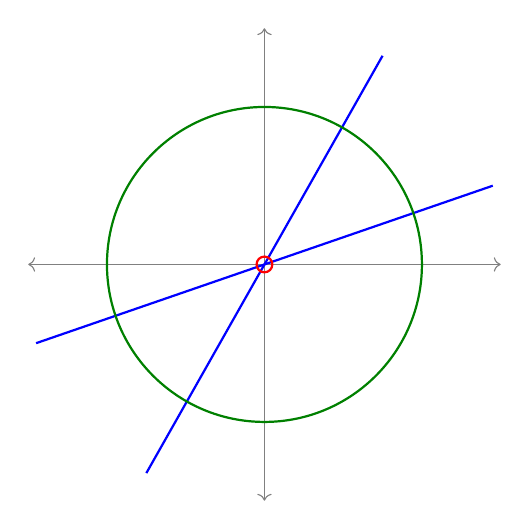
\begin{tikzpicture}
        % Grey x-y axis
        \draw[gray, <->] (-3,0) -- (3,0);
        \draw[gray, <->] (0,-3) -- (0,3);

        % Two generic blue lines intersecting at the origin
        \draw[blue, thick] (-2.9,-1) -- (2.9,1);
        \draw[blue, thick] (-1.5,-2.65) -- (1.5,2.65);

        \draw[red, thick] (0,0) circle (0.1);

        \draw<2->[green!50!black, thick] (0,0) circle (2);
    \end{tikzpicture}
    \end{center}
\end{frame}

\subsection{Hyperpolygon Space}
\begin{frame}[fragile]
    \frametitle{Hyperpolygon Space}
    \begin{wrapfigure}{r}[-5pt]{.25\textwidth}
    \vspace{-57pt}
    $
    \begin{tikzcd}[sep=large]
                    &1\arrow{d}{x_2}
                        %\arrow[rd, no head, thick, dotted, bend left, shorten <=3ex, shorten >=3ex]
                            &\\
        1\arrow{r}{x_3}  &2\arrow["y_1", r, dashed, bend left]\arrow["y_2", u, dashed, bend left]\arrow["y_3", l, dashed, bend left]\arrow["y_n", d, dashed, bend left]
                            &1\arrow{l}{x_1} \\
                    &1\arrow{u}{x_n}\arrow[lu, no head, thick, dotted, shorten <=3ex, shorten >=3ex, bend left=45, xshift=.4ex, yshift=.8ex]     &           \\
    \end{tikzcd}
    $
    \vspace{-80pt}
    \end{wrapfigure}
    Let $Q$ be the quiver shown to the right.  The space $X=\Rep Q$ is isomorphic to $T^*\Hom(\C^n,\C^2)\cong T^*\C^{2n}$ and has a standard hyperkähler structure $(X,g,I,\omega_I,\Omega_I)$.
    \vfill
    \pause
    The groups $G=\SU(2)\times\U(1)^n$ and $G_\C=\SL(2,\C)\times\GL(1,\C)^n$ act on $X$ and respectively preserve $\omega_I$ and $\Omega_I$.  The actions are hamiltonian, and admit moment maps $\mu_\R\from X\to\mathfrak g^*$ and $\mu_\C\from X\to\mathfrak g_\R^*$.
    \vfill
    \pause
    The moment maps decompose
        $$\mu_\C=\left(\mu_{\SL(2,\C)},\mu_{\GL(1,\C)^n}\right)\from X\to\mathfrak g_\C^*=\mathfrak{sl}(2,\C)^*\times(\C^n)^*$$
        $$\mu_\R=(\mu_{\SU(2)},\mu_{U(1)^n})\from X\to\mathfrak g^*=\mathfrak{su}(2)^*\times(\mathfrak u(1)^n)^*$$
    \vfill
\end{frame}

\begin{frame}
    \frametitle{Hyperpolygon Space}
    The moment maps decompose
        $$\mu_\C=\left(\mu_{\SL(2,\C)},\mu_{\GL(1,\C)^n}\right)\from X\to\mathfrak g_\C^*=\mathfrak{sl}(2,\C)^*\times(\C^n)^*$$
        $$\mu_\R=(\mu_{\SU(2)},\mu_{U(1)^n})\from X\to\mathfrak g^*=\mathfrak{su}(2)^*\times(\mathfrak u(1)^n)^*$$
    \vfill
    \begin{equation*}
        \mu_{\SL(2,\C)}(\bx,\by)=\sum_{i=1}^n (x_iy_i)_0,\qquad
            \mu_{\GL(1,\C)^n}(\bx,\by)=(y_1x_1,\dots,y_nx_n)
    \end{equation*}
    \begin{equation*}
        \mu_{\SU(2)}(\bx,\by)=\frac 12\sum_i (x_ix_i^\dagger)_0-(y_i^\dagger y_i)_0,\qquad
            \mu_{U(1)^n}=\frac 12\left(|x_i|^2-|y_i|^2\right)_{i=1}^n.
    \end{equation*}
    \vfill
    ($A_0$ denotes the trace-free part $A-\frac12\tr(A)\text{Id}$).
    \vfill

\end{frame}

\begin{frame}
    \frametitle{Hyperpolygon Space}
    Take $\tau=0\in Z(\mathfrak g_\C^*)$ and $\vec\beta\in Z(\mathfrak g^*)\cong\R^n$.  The hyperkähler quotient is
        $$\mathcal X(\vec\beta)=X\fourslash\limits_{(0,\vec\beta)}G=\left(\mu_\C^{-1}(0)\cap\mu_\R^{-1}(\vec\beta)\right)/G.$$
    Thus $\mathcal X(\vec\beta)$ is the \emph{moduli space of solutions to $\mu_\C=0$ and $\mu_\R=\vec\beta$ up to $G$-equivalence}.
    \vfill
    \pause
    Via the Kempf-Ness theorem, we can also regard $\mathcal X(\vec\beta)$ as the \emph{moduli space of $\vec\beta$-stable representations up to $G_\C$-equivalence}.
\end{frame}

\begin{frame}
    \frametitle{Hyperpolygon Space}
    The moment map equations have a geometric interpretation as ``telescoping polygons'' in $\mathfrak{su}(2)\cong\R^3$.  The equation $\mu_{\U(1)^n}(\bx,\by)=\vec\beta$ constrains the side lengths, and the equation $\mu_{\SU(2,\C)}(\bx,\by)=0$ ensures the polygon is closed.
    \vfill
    \begin{minipage}[t]{0.45\textwidth}
        \vspace{25pt}
        % Let $(\bx,\by)\in X=\Rep Q$,\\[2pt]
        % $\bx=(x_1,\dots,x_n)\in\Hom(\C,\C^2)^n$\\[2pt]
        % $\by=(y_1,\dots,y_n)\in\Hom(\C^2,\C)^n$\\[2pt]
        Set $v_i:=(x_ix_i^\dagger)_0$ and $w_i:=(y_i^\dagger y_i)_0$\\[1cm]
        $\mu_{\SU(2)}(\bx,\by)=\frac i2\sum v_i+w_i=0$\\[2pt]
        $\mu_{U(1)^n}(\bx,\by)=\frac i{\sqrt2}\left(|v_i|-|w_i|\right)=0$
        \vfill
    \end{minipage}
    \hfill
    \begin{minipage}[t]{0.45\textwidth}
        \vspace{-15pt}
        \begin{figure}
        \resizebox{4.5cm}{!}{
        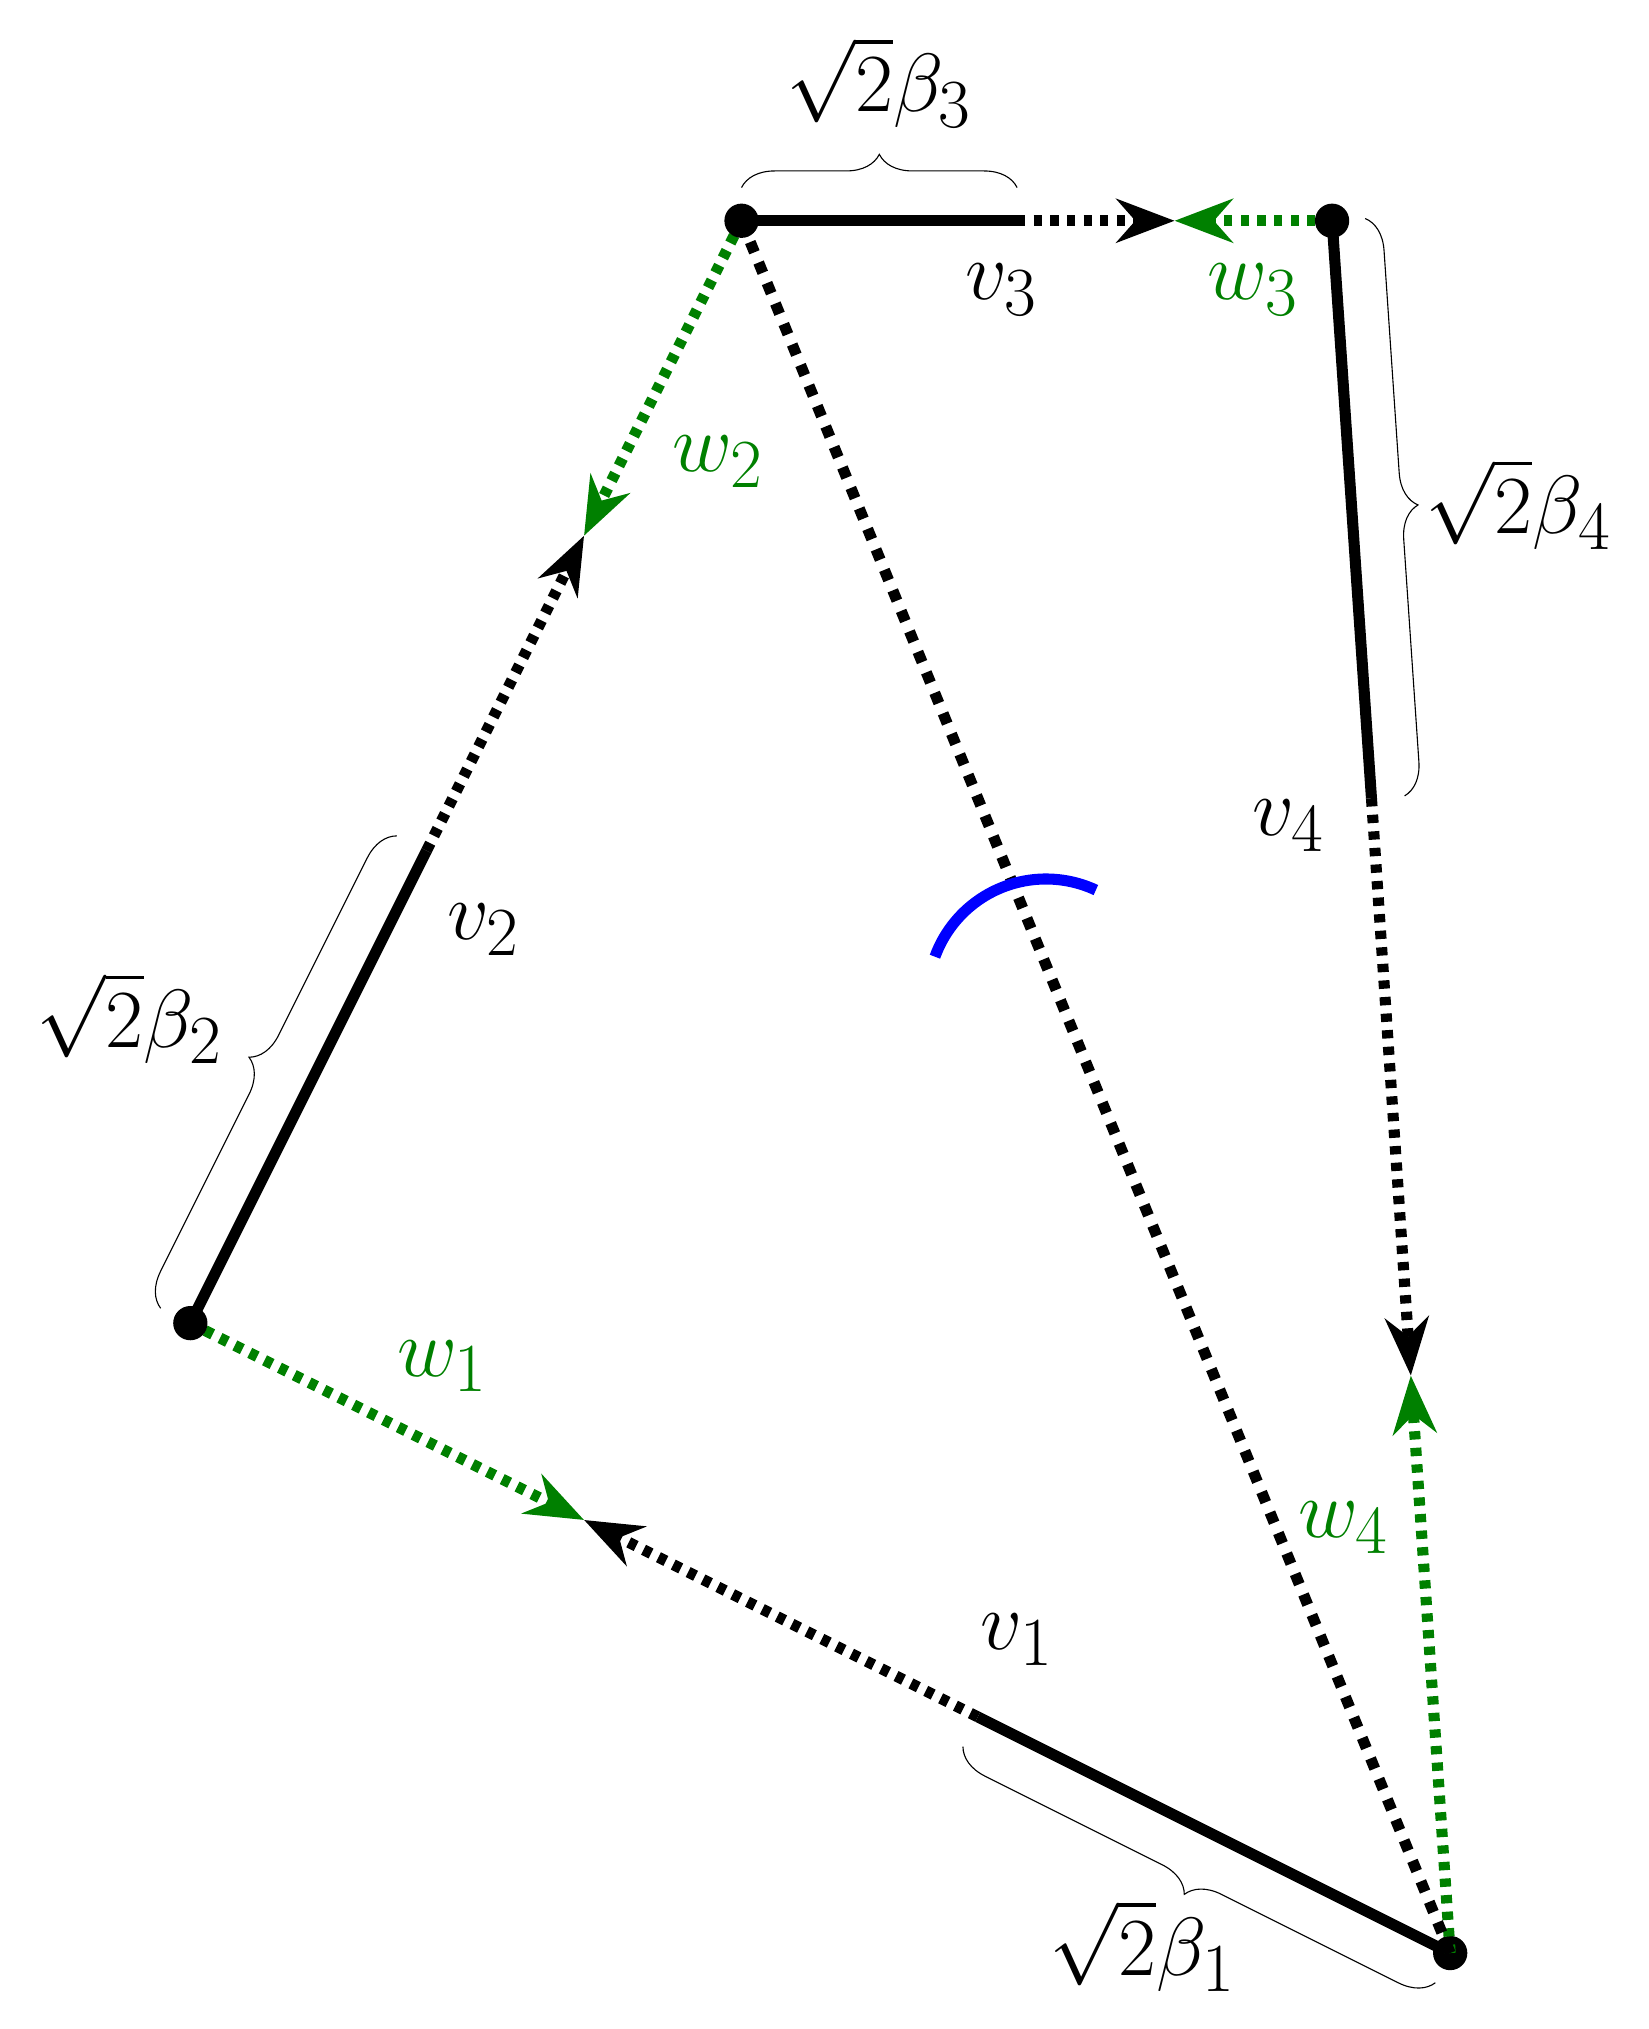
\begin{tikzpicture}
        \tikzstyle{every node}=[font=\LARGE]
        \draw [ fill=black , line width=1pt ] (16,2) circle (.2cm);
        \draw [line width=4pt] (16,2) -- (10,5);
            \draw [decorate, decoration = {brace,amplitude=12pt,raise=12pt}] (16,2) -- (10,5)
                node[midway,xshift=-6ex,yshift=-4em,font=\Huge]{\scalebox{1.2}{$\sqrt2\beta_1$}};
        \draw [line width=4pt, ->, >=Stealth, dashed] (10,5) -- (5,7.5);
            \node[font=\Huge, xshift=0em, yshift=3.5em] at (10.5,4.75) {\scalebox{1.2}{$v_1$}};
        \draw [ color=green!50!black, line width=4pt, ->, >=Stealth, dashed] (0,10) -- (5,7.5);
            \node[font=\Huge, xshift=2em, yshift=2em, color=green!50!black] at (2.5,8.75) {\scalebox{1.2}{$w_1$}};

        \draw [ fill=black , line width=1pt ] (0,10) circle (.2cm);
        \draw [line width=4pt] (0,10) -- (3,16);
            \draw [decorate, decoration = {brace,amplitude=12pt,raise=12pt}] (0,10) -- (3,16)
                node[midway,xshift=-15ex,yshift=2.5em,font=\Huge]{\scalebox{1.2}{$\sqrt2\beta_2$}};
        \draw [line width=4pt, ->, >=Stealth, dashed] (3,16) -- (5,20);
            \node[font=\Huge, xshift=3.5em, yshift=0em] at (2.5,15) {\scalebox{1.2}{$v_2$}};
        \draw [ color=green!50!black, line width=4pt, ->, >=Stealth, dashed] (7,24) -- (5,20);
            \node[font=\Huge, xshift=2em, yshift=-3em, color=green!50!black] at (6,22) {\scalebox{1.2}{$w_2$}};

        \draw [ fill=black , line width=1pt ] (7,24) circle (.2cm);
        \draw [line width=4pt] (7,24) -- (10.5,24);
            \draw [decorate, decoration = {brace,amplitude=12pt,raise=12pt}] (7,24) -- (10.5,24)
                node[midway,xshift=0ex,yshift=5em,font=\Huge]{\scalebox{1.2}{$\sqrt2\beta_3$}};
        \draw [line width=4pt, ->, >=Stealth, dashed] (10.5,24) -- (12.5,24);
            \node[font=\Huge, xshift=3em, yshift=-2.5em] at (9.25,24) {\scalebox{1.2}{$v_3$}};
        \draw [ color=green!50!black, line width=4pt, ->, >=Stealth, dashed] (14.5,24) -- (12.5,24);
            \node[font=\Huge, xshift=0em, yshift=-2.5em, color=green!50!black] at (13.5,24) {\scalebox{1.2}{$w_3$}};

        \draw [ fill=black , line width=1pt ] (14.5,24) circle (.2cm);
        \draw [line width=4pt] (14.5,24) -- (15, 24-22/3);
            \draw [decorate, decoration = {brace,amplitude=12pt,raise=12pt}] (14.5,24) -- (15, 24-22/3)
                node[midway,xshift=14ex,yshift=.2em,font=\Huge]{\scalebox{1.2}{$\sqrt2\beta_4$}};
        \draw [line width=4pt, ->, >=Stealth, dashed] (15, 24-22/3) -- (15.5, 24-2*22/3);
            \node[font=\Huge, xshift=-3em, yshift=-1em] at (15, 24-22/3) {\scalebox{1.2}{$v_4$}};
        \draw [ color=green!50!black, line width=4pt, ->, >=Stealth, dashed] (16,2) -- (15.5, 24-2*22/3);
            \node[font=\Huge, xshift=-3em, yshift=4em, color=green!50!black] at (15.7, 6) {\scalebox{1.2}{$w_4$}};

        %diagonal crease
        \draw [line width=4pt, loosely dotted] (16,2) -- (7,24);
        \draw [line width=4pt, blue] (11.5,15.5) arc (65:160:1.5);
        % \draw [line width=4pt, blue] (10.8,14.7) -- (11.5,15.5);
        % \draw [line width=4pt, blue] (10.8,14.7) -- (9.5,14.68);
        \end{tikzpicture}
        }
        \captionsetup{width = .8\textwidth}
        \caption{A hyperpolygon displayed as vectors in $\mathfrak{su}(2)\cong\R^3$}
        \label{fig: hyperpolygon}
        \end{figure}
    \end{minipage}
    \vfill
\end{frame}

\begin{frame}
    \frametitle{Hyperpolygon Space}
    Hyperpolygon space has real dimension $4(n-3)$ \cite{Kon02} and can be fibered over $\C^{n-3}$.  Pictured below is the $n=4$ hyperpolygon space:
    \vfill
    \begin{figure}
    \begin{center}
    \resizebox{5cm}{!}{
    \begin{tikzpicture}
        %R=1
            %Hitchin Base
                \draw (0,-8) ellipse (10cm and 2cm);
                %\node[below=12cm,font=\Huge]{\scalebox{1.8}{$R\to0$}};
            %Left torus
            \pic[rotate=0] at (-8.6,0) {opentorus={3.25cm}{7.5mm}{75}};
            %Line down
                \draw (-7,-4) -- (-7,-8);
            %Right torus
            \pic[rotate=0] at (5.4,0) {opentorus={3.25cm}{7.5mm}{75}};
            %Line down
                \draw (7,-4) -- (7,-8);
            %Central sphere
                \draw (0,0) circle (2cm);
                \draw (0,0) circle (2cm);
            %Top sphere
                %\draw (0,6) circle (4cm);
                \begin{axis}[axis x line = none, axis y line = none, width = 14cm, height = 8.8cm, at = {(-6.195cm,1.4cm)}]
                    \addplot[black, line width = 1.5pt]{x^2};
                \end{axis}
            %Left sphere
                \draw (-3,0) circle (1cm);
                \draw (-3,0) circle (1cm);
            %Bottom sphere
                \draw (0,-3) circle (1cm);
                \draw (0,-3) circle (1cm);
            %Right Sphere
                \draw (3,0) circle (1cm);
                \draw (3,0) circle (1cm);
            %Line down
                \draw (0,-4) -- (0,-8);
    \end{tikzpicture}
    }
    \end{center}
    \captionsetup{justification=centering}
    \caption{$n=4$ Hyperpolygon Space}
    \label{fig: degeneration}
    \end{figure}
\end{frame}

\subsection{Moduli Space of Parabolic Higgs Bundles}
\begin{frame}
    \frametitle{Parabolic Higgs Bundles}
    Let $C=\C\P^1$ and  $D=\{p_1,\dots,p_n\}$, and let $E=C\times\C^2$ be the trivial bundle with a \emph{parabolic structure} $(\mathcal F,\vec\alpha)$:
    $$
    \hspace{3.5cm}
    \begin{array}[column sep = -5pt]{ccccc}
        0   &\subset   &F_i             &\subset    &E_{p_i}\\[2pt]
        1   &>         &1-\alpha_i      &>          &\alpha_i
    \end{array}\qquad\qquad(i=1,\dots,n)
    $$
    We call $\vec\alpha\in(0,\frac12)^n$ the \emph{parabolic weights}.
    \vfill
    \pause
    A hermitian metric $h$ on $E$ is \emph{adapted} to $(\mathcal F,\vec\alpha)$ if the growth rate filtration on the stalks of $E$ at $p_i$ matches the filtration induced by $(\mathcal F_i,\alpha_i)$.
    $$\text{Ex:}\quad F_i=\langle e_1\rangle,\qquad h\sim\begin{pmatrix}|z-p_i|^{2(1-\alpha_i)}&|z-p_i|^{2\alpha_i}\\|z-p_i|^{2\alpha_i}&|z-p_i|^{2\alpha_i}\end{pmatrix}$$
\end{frame}

\begin{frame}
    \frametitle{Parabolic Higgs Bundles}
    Let $\mathcal E=(E,\delbar_\mathcal E,\mathcal F,\vec\alpha)$ be a parabolic bundle with a holomorphic structure.
    \vfill

    A \textit{strongly parabolic Higgs field} on $\mathcal E$ is a section $\varphi\in H^0(C,\End(E)\otimes K_{\C\P^1}(D))$ whose residues $\varphi_i\in\mathfrak{sl}(E_{p_i})$ are nilpotent with respect to $\mathcal F_i$:
        $$\varphi=\sum_{i=1}^n\frac{\varphi_i}{z-p_i}\de z\qquad\qquad\sum_{i=1}^n\varphi_i=0.$$
    \pause
    The parabolic weights determine a notion of $\vec\alpha$-stability for a Higgs bundle.
    \vfill

    We define $\mathcal M^\text{Higgs}(\vec\alpha)$ to be the moduli space of $\vec\alpha$-stable Higgs bundles up to gauge equivalence.  This gives $\mathcal M^\text{Higgs}(\vec\alpha)$ the structure of a holomorphic symplectic manifold.
    \vfill
\end{frame}

\begin{frame}
    \frametitle{Parabolic Higgs Bundles}
    \begin{theorem}[Non-Abelian Hodge Correspondence (NAHC)]
        Fix $R>0$.  A parabolic $\SL(2,\C)$-Higgs bundle $(E,\delbar_\mathcal E,\mathcal F,\vec\alpha,\varphi)$ is stable if and only if there exists a unique adapted metric $h_R$ (up to unitary equivalence) solving \emph{Hitchin's equations}
            \begin{align*}
                \mu_\C(\mathcal E,\varphi)&=\delbar_\mathcal E\varphi=0\\
                \mu_\R(\mathcal E,\varphi)&=R^{-1}F_{(\delbar_\mathcal E,h_R)}^\perp+R[\varphi^{\dagger_{h_R}},\varphi]=0
            \end{align*}
    \end{theorem}
    Such an $h_R$ is called the \emph{harmonic metric} for $(E,\delbar_\mathcal E,\mathcal F,\vec\alpha,\varphi)$.
    \vfill
    \pause
    The hyperkähler reduction process gives the moduli space an $\R_{>0}$-family of hyperkähler structures
        $$\mathcal M_R(\vec\alpha)=(\mathcal M^\text{Higgs}(\vec\alpha),\Omega,g_R).$$
    \vfill
    % \pause
    % For all $R>0$, $\mathcal M_R(\vec\alpha)$ is an ALG-$D_4$ gravitational instanton \cite{FMSW21}.
\end{frame}

\subsection{The Embedding}
\begin{frame}
    \frametitle{The Embedding}
    Godinho and Mandini \cite{GM11} produce an embedding $T_R\from\mathcal X(\vec\beta)\into\mathcal M_R(\vec\alpha)$ for $\vec\beta,\vec\alpha$ in appropriate chambers: given $(\bx,\by)\in\mathcal X(\vec\beta)$, the flag is $F_i=\langle x_i\rangle$ and the Higgs field residues are $\varphi_i=x_iy_i$.
    \vfill
    \begin{figure}
        \begin{center}
            \resizebox{8cm}{!}{
                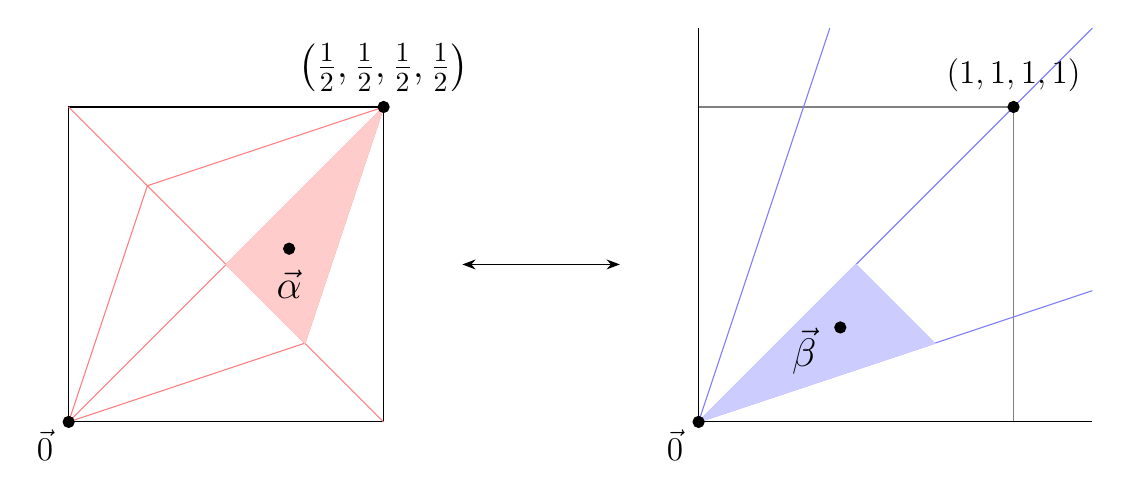
\begin{tikzpicture}
                    \draw (0,0) rectangle +(4cm,4cm);
                    \draw[red!50] (0,4) -- (4,0);
                    \draw[red!50] (0,0) -- (4,4);
                    \draw[red!50] (0,0) -- (3,1);
                    \draw[red!50] (3,1) -- (4,4);
                    \draw[red!50] (0,0) -- (1,3);
                    \draw[red!50] (1,3) -- (4,4);
                    \filldraw[red!20] (2,2) -- (3,1) -- (4,4) -- cycle;
                    \filldraw (2.8,2.2) circle (2pt)
                    node[below=1.5mm]{\Large$\vec\alpha$};
                    %\draw[line width=2pt,->,>=Stealth,dashed] (2.8,2.2) -- (4,4);
                    \filldraw (0,0) circle (2pt);
                    \filldraw (4,4) circle (2pt);
        \node[xshift = -3mm, yshift = -3mm] at (0,0) {\large$\vec0$};    
        \node[xshift = 0mm, yshift = 5mm] at (4,4) {\Large$\left(\frac12,\frac12,\frac12,\frac12\right)$};
        
        \draw[<->, >=Stealth] (5,2) -- (7,2);
        
        \draw[black!50] (8,0) rectangle +(4cm,4cm);
        \draw (8,0) -- (13,0);
        \draw (8,0) -- (8,5);
        \draw[blue!50] (8,0) -- (13,5);
        \draw[blue!50] (8,0) -- (13,5/3);
        \draw[blue!50] (8,0) -- (8+5/3,5);
        \filldraw[blue!20] (8,0) -- (10,2) -- (11,1) -- cycle;
        \filldraw (9.8,1.2) circle (2pt)
        node[below=3mm,left=1.8mm]{\Large$\vec\beta$};
        \filldraw (8,0) circle (2pt);
        \filldraw (12,4) circle (2pt);
        \node[xshift = -3mm, yshift = -3mm] at (8,0) {\large$\vec0$};    
        \node[xshift = 0mm, yshift = 4mm] at (12,4) {\large$(1,1,1,1)$};
                \end{tikzpicture}
            }
        \end{center}
        \caption{Chamber Structures}
    \end{figure}
    \vfill
    This embedding is open and dense, and respects the holomorphic symplectic structures but not the full hyperkähler metrics.
    \vfill
\end{frame}

\section{Metric Degeneration}
\subsection{Hitchin Fibration}
\begin{frame}
    \frametitle{Metric Degeneration}
    \begin{wrapfigure}{r}[-10pt]{4cm}
    \vspace{-30pt}
    \begin{center}
    \resizebox{4cm}{!}{
    \begin{tikzpicture}
        %R=1
            %Hitchin Base
                \draw (0,-8) ellipse (10cm and 2cm);
            %Left torus
                \pic[rotate=-90] at (-6,0) {torus={3.25cm}{7.5mm}{72}};
            %Line down
                \draw (-6,-4) -- (-6,-8);
            %Right torus
                \pic[rotate=-90] at (6,0) {torus={3.25cm}{7.5mm}{76}};
            %Line down
                \draw (6,-4) -- (6,-8);
            %Central sphere
                \draw (0,0) circle (2cm);
                \shade[ball color = green!60, opacity = 0.7] (0,0) circle (2cm);
            %Top sphere
                \draw (0,3) circle (1cm);
                \shade[ball color = green!60, opacity = 0.7] (0,3) circle (1cm);
            %Left sphere
                \draw (-3,0) circle (1cm);
                \shade[ball color = green!60, opacity = 0.7] (-3,0) circle (1cm);
            %Bottom sphere
                \draw (0,-3) circle (1cm);
                \shade[ball color = green!60, opacity = 0.7] (0,-3) circle (1cm);
            %Right Sphere
                \draw (3,0) circle (1cm);
                \shade[ball color = green!60, opacity = 0.7] (3,0) circle (1cm);
            %Line down
                \draw (0,-4) -- (0,-8);
    \end{tikzpicture}
    }
    \end{center}
    \captionsetup{justification=centering}
    \caption{Hitchin Fibration when $n=4$}
    \vspace{-60pt}
    \end{wrapfigure}
    For $n=4$, the \textit{Hitchin fibration} is a map $\mathcal H\from\mathcal M_R(\vec\alpha)\to\C$\\ given by $(\mathcal E,\varphi)\mapsto\det\varphi$.
    \vfill
    \pause
    The fibers are generically holomorphic Lagrangian\\ tori of volume $4\pi^2/R$, but the singular fiber $\mathcal H^{-1}(0)$ is five\\ 2-spheres which generate $H_2(\mathcal M_R(\vec\alpha),\Z)$.
    \vfill
    \pause
    Taking $R\to0$ enlarges the fibers while shrinking the base.
\end{frame}

\subsection{Chamber Walls}
\begin{frame}
    \frametitle{Metric Degeneration}
    On the other hand, varying $\vec\alpha$ within its chamber also modifies the hyperkähler structure without changing the notion of $\vec\alpha$-stability.
    \vfill
    \pause
    This is reflected in the period data, also called the \textit{Torelli numbers}, which are calculated by integrating $\omega_{I,R}$ on generators of $H_2(\mathcal M_R(\vec\alpha),\C)$.
    \vfill
    \pause
    The chamber walls are the values of $\vec\alpha\in(0,\frac12)^n$ for which the respective Torelli numbers vanish, resulting in singularities in $\mathcal M_R(\vec\alpha)$.
    \vfill
    \begin{figure}
        \begin{center}
        \resizebox{4cm}{!}{
            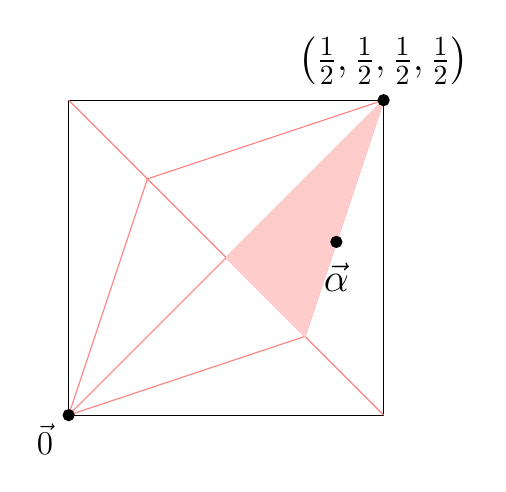
\begin{tikzpicture}
                \draw (0,0) rectangle +(4cm,4cm);
                \draw[red!50] (0,4) -- (4,0);
                \draw[red!50] (0,0) -- (4,4);
                \draw[red!50] (0,0) -- (3,1);
                \draw[red!50] (3,1) -- (4,4);
                \draw[red!50] (0,0) -- (1,3);
                \draw[red!50] (1,3) -- (4,4);
                \filldraw[red!20] (2,2) -- (3,1) -- (4,4) -- cycle;
                \filldraw (3.4,2.2) circle (2pt)
                node[below=1.5mm]{\Large$\vec\alpha$};
                %\draw[line width=2pt,->,>=Stealth,dashed] (2.8,2.2) -- (4,4);
                \filldraw (0,0) circle (2pt);
                \filldraw (4,4) circle (2pt);
                \node[xshift = -3mm, yshift = -3mm] at (0,0) {\large$\vec0$};    
                \node[xshift = 0mm, yshift = 5mm] at (4,4) {\Large$\left(\frac12,\frac12,\frac12,\frac12\right)$};
            \end{tikzpicture}
            }
        \resizebox{4cm}{!}{
        \begin{tikzpicture}
        %R=1
            %Hitchin Base
                \draw (0,-8) ellipse (10cm and 2cm);
            %Left torus
                \pic[rotate=-90] at (-6,0) {torus={3.25cm}{7.5mm}{72}};
            %Line down
                \draw (-6,-4) -- (-6,-8);
            %Right torus
                \pic[rotate=-90] at (6,0) {torus={3.25cm}{7.5mm}{76}};
            %Line down
                \draw (6,-4) -- (6,-8);
            %Central sphere
                \draw (0,0) circle (2cm);
                \shade[ball color = green!60, opacity = 0.7] (0,0) circle (2cm);
            %Top sphere
                \draw (0,3) circle (1cm);
                \shade[ball color = green!60, opacity = 0.7] (0,3) circle (1cm);
            %Left sphere
                \draw (-3,0) circle (1cm);
                \shade[ball color = green!60, opacity = 0.7] (-3,0) circle (1cm);
            %Bottom sphere
                \draw (0,-3) circle (1cm);
                \shade[ball color = green!60, opacity = 0.7] (0,-3) circle (1cm);
            %Right Sphere
                \filldraw (2.1,0) circle (3pt);
                % \shade[ball color = green!60, opacity = 0.7] (3,0) circle (1cm);
            %Line down
                \draw (0,-4) -- (0,-8);
            \end{tikzpicture}
        }
        \end{center}


        \caption{Chamber Structures}
    \end{figure}

\end{frame}

\subsection{Main Theorem}
\begin{frame}
    \frametitle{Metric Degeneration}
    By letting $\alpha_i(R)=\frac12-R\beta_i$, we produce a family  of moduli spaces $\mathcal M_R:=\mathcal M_R(\vec\alpha(R))$ in which four of the five Torelli numbers are fixed, while the last grows without bound as $R\to0$.
    \vfill
    \onslide<2->
    \begin{theorem}[Fredrickson\,-Y; Heller-Heller-Meneses]\label{thm: main theorem}
        As $R\to0$, the family of metrics $g_R$ converges pointwise to the metric $2\pi g_\mathrm{HP}$ on the restriction to the image of $\mathcal T_R\from\mathcal X(\vec\beta)\into\mathcal M_R(\vec\alpha(R))$.  In other words, $\lim\limits_{R\to0}\mathcal T_R^*(g_R)=2\pi g_\mathrm{HP}$.
    \end{theorem}
    \onslide<1->
    \begin{figure}
    \begin{center}
    \resizebox{12cm}{!}{
    \begin{tikzpicture}
        %R=1
            %Hitchin Base
                \draw (0,-8) ellipse (10cm and 2cm)
                node[below=3cm,font=\Huge]{\scalebox{1.8}{$R=1$}};
            %Left torus
                \pic[rotate=-90] at (-6,0) {torus={3.25cm}{7.5mm}{72}};
            %Line down
                \draw (-6,-4) -- (-6,-8);
            %Right torus
                \pic[rotate=-90] at (6,0) {torus={3.25cm}{7.5mm}{76}};
            %Line down
                \draw (6,-4) -- (6,-8);
            %Central sphere
                \draw (0,0) circle (2cm);
                \shade[ball color = green!60, opacity = 0.7] (0,0) circle (2cm);
            %Top sphere
                \draw (0,3) circle (1cm);
                \shade[ball color = green!60, opacity = 0.7] (0,3) circle (1cm);
            %Left sphere
                \draw (-3,0) circle (1cm);
                \shade[ball color = green!60, opacity = 0.7] (-3,0) circle (1cm);
            %Bottom sphere
                \draw (0,-3) circle (1cm);
                \shade[ball color = green!60, opacity = 0.7] (0,-3) circle (1cm);
            %Right Sphere
                \draw (3,0) circle (1cm);
                \shade[ball color = green!60, opacity = 0.7] (3,0) circle (1cm);
            %Line down
                \draw (0,-4) -- (0,-8);

        %R=.5
            %Hitchin Base
                \draw (24,-8) ellipse (10cm and 2cm)
                node[below=3cm,font=\Huge]{\scalebox{1.8}{$R=0.5$}};
            %Left torus
                \pic[rotate=-90] at (18,1) {torus={4.1cm}{9mm}{74}};
            %Line down
                \draw (18,-4) -- (18,-8);
                %Central sphere
                \draw (24,0) circle (2cm);
                \shade[ball color = green!60, opacity = 0.7] (24,0) circle (2cm);
                %Top sphere
                \draw (24,4) circle (2cm);
                \shade[ball color = green!60, opacity = 0.7] (24,4) circle (2cm);
                %Left sphere
                \draw (21,0) circle (1cm);
                \shade[ball color = green!60, opacity = 0.7] (21,0) circle (1cm);
                %Bottom sphere
                \draw (24,-3) circle (1cm);
                \shade[ball color = green!60, opacity = 0.7] (24,-3) circle (1cm);
                %Right Sphere
                \draw (27,0) circle (1cm);
                \shade[ball color = green!60, opacity = 0.7] (27,0) circle (1cm);
                %Line down
                \draw (24,-4) -- (24,-8);
                %Right torus
                    \pic[rotate=-90] at (30,1) {torus={4.1cm}{9mm}{77}};
                %Line down
                    \draw (30,-4) -- (30,-8);
        

        %R->0
            %Hitchin Base
                \draw (48,-8) ellipse (10cm and 2cm)
                node[below=3cm,font=\Huge]{\scalebox{1.8}{$R\to0$}};
            %Left torus
            \pic[rotate=0] at (39.4,0) {opentorus={3.25cm}{7.5mm}{75}};
            %Line down
                \draw (41,-4) -- (41,-8);
            %Right torus
            \pic[rotate=0] at (53.4,0) {opentorus={3.25cm}{7.5mm}{75}};
            %Line down
                \draw (55,-4) -- (55,-8);
            %Central sphere
                \draw (48,0) circle (2cm);
                \shade[ball color = green!60, opacity = 0.7] (48,0) circle (2cm);
            %Top sphere
                %\draw (0,6) circle (4cm);
                \shade[ball color = green!60, opacity = 0.5] (48,3) circle (1cm);
                \shade[ball color = green!60, opacity = 0.4] (48,4) circle (2cm);
                \shade[ball color = green!60, opacity = 0.4] (48,5) circle (3cm);
                \begin{axis}[axis x line = none, axis y line = none, width = 14cm, height = 8.8cm, at = {(41.805cm,1.4cm)}]
                    \addplot[black, line width = 1.5pt]{x^2};
                \end{axis}
            %Left sphere
                \draw (45,0) circle (1cm);
                \shade[ball color = green!60, opacity = 0.7] (45,0) circle (1cm);
            %Bottom sphere
                \draw (48,-3) circle (1cm);
                \shade[ball color = green!60, opacity = 0.7] (48,-3) circle (1cm);
            %Right Sphere
                \draw (51,0) circle (1cm);
                \shade[ball color = green!60, opacity = 0.7] (51,0) circle (1cm);
            %Line down
                \draw (48,-4) -- (48,-8);
    \end{tikzpicture}
    }
    \end{center}
    \caption{Degenerate Limit as $R\to0$, ($n=4$ case)}
    \end{figure}
\end{frame}


\section{Broader Context}
\subsection{Gravitational Instantons}
\begin{frame}
    \frametitle{Gravitational Instantons}
    \begin{definition}
        A \emph{gravitational instanton} is a complete noncompact hyperkähler 4-manifold satisfying the finite energy condition
            $$\int|\text{Rm}|^2<\infty.$$
    \end{definition}
    \pause
    G.\ Chen and X.\ Chen \cite{CC21,CC17,CC20} provide a full classification according to the asymptotic behavior at the noncompact ends.
    \vfill
\end{frame}

\begin{frame}
    \frametitle{Gravitational Instantons}
    At infinity, a gravitational instanton $X$ has the form $\left(\R^{4-m}\times\mathbb T^m\right)/\Gamma$ for $m=0,1,2,3$ and $\Gamma\subset\SU(2)$. Depending on $m$, we say $X$ is:
    $$
    \setlength\arraycolsep{0pt}
    \begin{array}{lc}
        \text{ALE}\quad &m=0\\
        \text{ALF}\quad &m=1\\
        \text{ALG}^{(*)}\quad &m=2\\
        \text{ALH}^{(*)}\quad &m=3
    \end{array}$$
    (the star appears if $|\text{Rm}|\notin O(r^{-2+\eps})$ for any $\eps>0$.)
    \vfill
    \pause
    When $n=4$, hyperpolygon space $\mathcal X(\vec\beta)$ is an ALE-$D_4$ gravitational instanton \cite{Nak94}, and the Higgs bundle moduli space $\mathcal M_R(\vec\alpha)$ is an ALG-$D_4$ instanton \cite{FMSW21}.
    \vfill
    \begin{figure}
    \begin{center}
    \resizebox{7.5cm}{!}{
    \begin{tikzpicture}
        %R=1
            %Hitchin Base
                \draw (0,-8) ellipse (10cm and 2cm);
                %\node[below=12cm,font=\Huge]{\scalebox{1.8}{$R\to0$}};
            %Left torus
            \pic[rotate=0] at (-8.6,0) {opentorus={3.25cm}{7.5mm}{75}};
            %Line down
                \draw (-7,-4) -- (-7,-8);
            %Right torus
            \pic[rotate=0] at (5.4,0) {opentorus={3.25cm}{7.5mm}{75}};
            %Line down
                \draw (7,-4) -- (7,-8);
            %Central sphere
                \draw (0,0) circle (2cm);
                \draw (0,0) circle (2cm);
            %Top sphere
                %\draw (0,6) circle (4cm);
                \begin{axis}[axis x line = none, axis y line = none, width = 14cm, height = 8.8cm, at = {(-6.195cm,1.4cm)}]
                    \addplot[black, line width = 1.5pt]{x^2};
                \end{axis}
            %Left sphere
                \draw (-3,0) circle (1cm);
                \draw (-3,0) circle (1cm);
            %Bottom sphere
                \draw (0,-3) circle (1cm);
                \draw (0,-3) circle (1cm);
            %Right Sphere
                \draw (3,0) circle (1cm);
                \draw (3,0) circle (1cm);
            %Line down
                \draw (0,-4) -- (0,-8);
    \end{tikzpicture}
    \hspace{10cm}
    \begin{tikzpicture}
        %R=1
            %Hitchin Base
                \draw (0,-8) ellipse (10cm and 2cm);
            %Left torus
                \pic[rotate=-90] at (-6,0) {torus={3.25cm}{7.5mm}{72}};
            %Line down
                \draw (-6,-4) -- (-6,-8);
            %Right torus
                \pic[rotate=-90] at (6,0) {torus={3.25cm}{7.5mm}{76}};
            %Line down
                \draw (6,-4) -- (6,-8);
            %Central sphere
                \draw (0,0) circle (2cm);
                %\shade[ball color = green!60, opacity = 0.7] (0,0) circle (2cm);
            %Top sphere
                \draw (0,3) circle (1cm);
                %\shade[ball color = green!60, opacity = 0.7] (0,3) circle (1cm);
            %Left sphere
                \draw (-3,0) circle (1cm);
                %\shade[ball color = green!60, opacity = 0.7] (-3,0) circle (1cm);
            %Bottom sphere
                \draw (0,-3) circle (1cm);
                %\shade[ball color = green!60, opacity = 0.7] (0,-3) circle (1cm);
            %Right Sphere
                \draw (3,0) circle (1cm);
                %\shade[ball color = green!60, opacity = 0.7] (3,0) circle (1cm);
            %Line down
                \draw (0,-4) -- (0,-8);
    \end{tikzpicture}
    }
    \end{center}
    \captionsetup{justification=centering}
    \caption{$\mathcal X(\vec\beta)$ on the left, $\mathcal M(\vec\alpha)$ on the right}
    \label{fig: degeneration}
    \end{figure}
\end{frame}

\begin{frame}
    \frametitle{Classic Example of Instanton Degeneration}
    \vspace{-10pt}
    The ALF-$A_n$ instantons have explicit metric descriptions using Gibbons-Hawking potentials on a principal $\U(1)$-bundle over $\R^3$
        $$V_t(x)=t+\frac1{4\pi\prod_{i=0}^n|x-p_i|}$$
    \onslide<2->
    By degenerating $t\to0$, the ALF-$A_n$ metrics converge to an ALE-$A_n$ metric.
    \vfill
    \onslide<1->
    \begin{wrapfigure}{l}[8pt]{8cm}
    \vspace{-35pt}
    \includegraphics[width=9cm]{ALF-An Degeneration.png}
    \caption{ALF-$A_1$ instanton}
    \end{wrapfigure}
    %$$\quad$$
    $$\frac1{V_t(x)}=\frac{4\pi\prod|x-p_i|}{4\pi t\prod|x-p_i|+1}$$
    \vspace{1cm}
\end{frame}

\subsection{K3 Bubbling Limits}
\begin{frame}
    \frametitle{Bubbling Limits}
    Gravitational instantons appear as bubbling limits of degenerating K3 surfaces by ``zooming in'' as a singularity develops.
    \vfill
    \begin{figure}
    \includegraphics[width=10cm]{Bubbling Phenomenon.png}
    \caption{Example of bubbling limits}
    \end{figure}
    \vfill
    \pause
    Studying degenerations between instantons lends insight towards the boundary faces of the moduli of K3 surfaces.
    \vfill
    \pause
    Theorem 1 is thus one step in a larger story about how the various boundary faces meet each other.
    \vfill
\end{frame}


\begin{frame}
    \frametitle{Other Instanton Degenerations}
    \begin{figure}
    \includegraphics[width=9cm]{Cherkis Degeneration Diagram.png}
    \caption{Conjectured Instanton Degenerations (by Sergey Cherkis)}
    \end{figure}
\end{frame}


\section{Proof of Main Theorem}
\begin{frame}
    \frametitle{Theorem Statement}
    \begin{theorem}
        As $R\to0$, the family of metrics $g_R$ converges pointwise to the metric $2\pi g_\mathrm{HP}$ on the restriction to the image of $\mathcal T_R\from\mathcal X(\vec\beta)\into\mathcal M_R(\vec\alpha(R))$.  In other words, $\lim_{R\to0}\mathcal T_R^*(g_R)=2\pi g_\mathrm{HP}$.
    \end{theorem}
    \begin{figure}
    \begin{center}
    \resizebox{12cm}{!}{
    \begin{tikzpicture}
        %R=1
            %Hitchin Base
                \draw (0,-8) ellipse (10cm and 2cm)
                node[below=3cm,font=\Huge]{\scalebox{1.8}{$R=1$}};
            %Left torus
                \pic[rotate=-90] at (-6,0) {torus={3.25cm}{7.5mm}{72}};
            %Line down
                \draw (-6,-4) -- (-6,-8);
            %Right torus
                \pic[rotate=-90] at (6,0) {torus={3.25cm}{7.5mm}{76}};
            %Line down
                \draw (6,-4) -- (6,-8);
            %Central sphere
                \draw (0,0) circle (2cm);
                \shade[ball color = green!60, opacity = 0.7] (0,0) circle (2cm);
            %Top sphere
                \draw (0,3) circle (1cm);
                \shade[ball color = green!60, opacity = 0.7] (0,3) circle (1cm);
            %Left sphere
                \draw (-3,0) circle (1cm);
                \shade[ball color = green!60, opacity = 0.7] (-3,0) circle (1cm);
            %Bottom sphere
                \draw (0,-3) circle (1cm);
                \shade[ball color = green!60, opacity = 0.7] (0,-3) circle (1cm);
            %Right Sphere
                \draw (3,0) circle (1cm);
                \shade[ball color = green!60, opacity = 0.7] (3,0) circle (1cm);
            %Line down
                \draw (0,-4) -- (0,-8);


            %Left torus attempt
            % \node at (-6,0) {
            % \begin{tikzpicture}[xscale=.4]
            %     \draw[double distance = 1.2cm] (90:2) arc (90:270:2);
            %     \draw[double distance = 1.2cm] (-90:2) arc (-90:90:2);
            % \end{tikzpicture}
            % };



        %R=.5
            %Hitchin Base
                \draw (24,-8) ellipse (10cm and 2cm)
                node[below=3cm,font=\Huge]{\scalebox{1.8}{$R=0.5$}};
            %Left torus
                \pic[rotate=-90] at (18,1) {torus={4.1cm}{9mm}{74}};
            %Line down
                \draw (18,-4) -- (18,-8);
                %Central sphere
                \draw (24,0) circle (2cm);
                \shade[ball color = green!60, opacity = 0.7] (24,0) circle (2cm);
                %Top sphere
                \draw (24,4) circle (2cm);
                \shade[ball color = green!60, opacity = 0.7] (24,4) circle (2cm);
                %Left sphere
                \draw (21,0) circle (1cm);
                \shade[ball color = green!60, opacity = 0.7] (21,0) circle (1cm);
                %Bottom sphere
                \draw (24,-3) circle (1cm);
                \shade[ball color = green!60, opacity = 0.7] (24,-3) circle (1cm);
                %Right Sphere
                \draw (27,0) circle (1cm);
                \shade[ball color = green!60, opacity = 0.7] (27,0) circle (1cm);
                %Line down
                \draw (24,-4) -- (24,-8);
                %Right torus
                    \pic[rotate=-90] at (30,1) {torus={4.1cm}{9mm}{77}};
                %Line down
                    \draw (30,-4) -- (30,-8);
        

        %R->0
            %Hitchin Base
                \draw (48,-8) ellipse (10cm and 2cm)
                node[below=3cm,font=\Huge]{\scalebox{1.8}{$R\to0$}};
            %Left torus
            \pic[rotate=0] at (39.4,0) {opentorus={3.25cm}{7.5mm}{75}};
            %Line down
                \draw (41,-4) -- (41,-8);
            %Right torus
            \pic[rotate=0] at (53.4,0) {opentorus={3.25cm}{7.5mm}{75}};
            %Line down
                \draw (55,-4) -- (55,-8);
            %Central sphere
                \draw (48,0) circle (2cm);
                \shade[ball color = green!60, opacity = 0.7] (48,0) circle (2cm);
            %Top sphere
                %\draw (0,6) circle (4cm);
                \shade[ball color = green!60, opacity = 0.5] (48,3) circle (1cm);
                \shade[ball color = green!60, opacity = 0.4] (48,4) circle (2cm);
                \shade[ball color = green!60, opacity = 0.4] (48,5) circle (3cm);
                \begin{axis}[axis x line = none, axis y line = none, width = 14cm, height = 8.8cm, at = {(41.805cm,1.4cm)}]
                    \addplot[black, line width = 1.5pt]{x^2};
                \end{axis}
            %Left sphere
                \draw (45,0) circle (1cm);
                \shade[ball color = green!60, opacity = 0.7] (45,0) circle (1cm);
            %Bottom sphere
                \draw (48,-3) circle (1cm);
                \shade[ball color = green!60, opacity = 0.7] (48,-3) circle (1cm);
            %Right Sphere
                \draw (51,0) circle (1cm);
                \shade[ball color = green!60, opacity = 0.7] (51,0) circle (1cm);
            %Line down
                \draw (48,-4) -- (48,-8);
        % %R=.1
        %     %Hitchin Base
        %         \draw (48,-8) ellipse (10cm and 2cm)
        %         node[below=3cm,font=\Huge]{\scalebox{1.8}{$R\to0$}};
        %     %Left torus
        %         \pic[rotate=-90] at (42,3) {torus={5.7cm}{12mm}{74}};
        %     %Line down
        %         \draw (42,-4) -- (42,-8);
        %         %Central sphere
        %         \draw (48,0) circle (2cm);
        %         \shade[ball color = green!60, opacity = 0.7] (48,0) circle (2cm);
        %         %Top sphere
        %         \draw (48,6) circle (4cm);
        %         \shade[ball color = green!60, opacity = 0.7] (48,6) circle (4cm);
        %         %Left sphere
        %         \draw (45,0) circle (1cm);
        %         \shade[ball color = green!60, opacity = 0.7] (45,0) circle (1cm);
        %         %Bottom sphere
        %         \draw (48,-3) circle (1cm);
        %         \shade[ball color = green!60, opacity = 0.7] (48,-3) circle (1cm);
        %         %Right Sphere
        %         \draw (51,0) circle (1cm);
        %         \shade[ball color = green!60, opacity = 0.7] (51,0) circle (1cm);
        %         %Line down
        %         \draw (48,-4) -- (48,-8);
        %         %Right torus
        %             \pic[rotate=-90] at (54,3) {torus={5.7cm}{12mm}{77}};
        %         %Line down
        %             \draw (54,-4) -- (54,-8);
    \end{tikzpicture}
    }
    \end{center}
    \caption{Degenerate Limit as $R\to0$, ($n=4$ case)}
    \end{figure}
\end{frame}


\begin{frame}
    \frametitle{Proof Strategy}
    To calculate the pullback $\mathcal T_R^*(g_R)$, we evaluate $g_R$ on the pushforward of tangent vectors.  Given a 1-parameter family $(\bx(t),\by(t))\in\mathcal X(\vec\beta)$, we use $\mathcal T_R$ and the NAHC to produce
    \begin{align*}
        (\bx(t),\by(t))
            \xmapsto[\mathcal T_R]{}(\delbar,\varphi(t),\mathcal F(t),h_R(t))
            \xmapsto[\text{gauge change}]{}(A_R(t),\Phi_R(t),\mathcal F(0),h_R(0))
    \end{align*}
    which solves Hitchin's equations for all $t$.
    \vfill
    \pause
    Then we isolate the first variations and calculate
        $$\|(\dot A_R,\dot\Phi_R)\|_{g_R}^2=\int_C R^{-1}|\dot A_R|_{h_R}^2+R|\dot\Phi_R|_{h_R}^2\xrightarrow[R\to0]{\mathrm{(goal)}}2\pi\sum_{i=1}^n|\dot x_i|^2+|\dot y_i|^2.$$
\end{frame}


\begin{frame}
    \frametitle{Proof Strategy}
    The proof requires information about the family of harmonic metrics $h_R$.  Solving Hitchin's equation explicitly is infeasible, but the limiting behavior can be understood.
    \vfill
    \pause
    The main challenge was reconciling the effects of degenerating the parameter $R$ in Hitchin's equation with those of taking the limit $\vec\alpha(R')\to(\frac12,\dots,\frac12)$.  It is precisely the relative rates at which $R$ and $R'$ approach 0 that encodes the data from $\vec\beta$.
    \vfill
    \pause
    \begin{wrapfigure}{r}{5cm}
    \vspace{-45pt}
    \resizebox{4cm}{!}{
    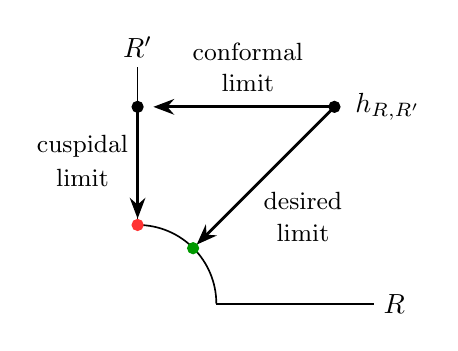
\begin{tikzpicture}
        %right branch
        \draw[line width = .6pt] (1,0) -- (3,0);
        \node[right=3cm]{$R$};
        %up branch
        \draw[line width = .6pt] (0,1) -- (0,3);
        \node[above=3cm]{$R'$};
        %arc
        \draw[line width = .6pt] (1,0) arc (0:90:1);
        %conformal limit
        \draw[line width=1pt, ->, >=Stealth] (2.5,2.5) -- (0.2,2.5);
        \node[font=\small] at (1.4,3.2) {conformal};
        \node[font=\small] at (1.4,2.8) {limit};
        \filldraw[black] (0,2.5) circle (2pt);
        %KW limit
        \draw[black, line width=1pt, ->, >=Stealth] (0,2.5) -- (0,1.08);
        \node[font=\small] at (-.7,2.0) {cuspidal};
        \node[font=\small] at (-.7,1.6) {limit};
        \filldraw[red!80] (0,1) circle (2pt);
        %desired limit
        \draw[black, line width=1pt, ->, >=Stealth] (2.5,2.5) -- (1.5/2,1.5/2);
        \filldraw[green!60!black] (1.41/2,1.41/2) circle (2pt);
        \node[font=\small] at (2.1,1.3) {desired};
        \node[font=\small] at (2.1,0.9) {limit};
        %alpha(1)
        \filldraw[black] (2.5,2.5) circle (2pt)
        node[right=4pt]{$h_{R,R'}$};
    \end{tikzpicture}
    }
    \captionsetup{justification=centering}
    \caption{Micro-Scale Analysis as $R\to0$ and $R'\to0$}
    \end{wrapfigure}
    We capture data from the relative rates by constructing\\ local model metrics, and we glue them to produce a\\ global metric.  Then we perturb to an actual solution\\ using an implicit function theorem argument.
    \vfill
\end{frame}
% \begin{frame}
%     Given a 1-parameter family $(\bx(t),\by(t))\in\mathcal X(\vec\beta)$, we use $\mathcal T_R$ and the NAHC to produce
%     \begin{align*}
%         (\bx(t),\by(t))
%             \xmapsto[\mathcal T_R]{}(\delbar,\mathcal F(t),\varphi(t),h_R(t))
%             \xmapsto[\text{gauge change}]{}(A_R(t),\Phi_R(t))
%     \end{align*}
%     where the last bundle solves Hitchin's equations with $h_R(0)$.
%     \vfill
%     \pause
%     Then we isolate the first variations and calculate
%         $$\|(\dot A_R,\dot\Phi_R)\|_{g_R}^2=\int_C R^{-1}|\dot A_R|_{h_R}^2+R|\dot\Phi_R|_{h_R}^2\xrightarrow[R\to0]{}2\pi\sum_{i=1}^4|\dot x_i|^2+|\dot y_i|^2$$
% \end{frame}

\subsection{Local Models}
\begin{frame}
    \frametitle{Local Models}
    Fix $i\in\{1,\dots,n\}$ and recall
        $$0=\mu_{\C^\times\!,i\,}(\bx,\by)=y_ix_i,\qquad\beta_i=\mu_{\U(1),i\,}(\bx,\by)=\frac 12(|x_i|^2-|y_i|^2)$$
    Locally, we have the parabolic structure
    $$
    \begin{array}[column sep = -5pt]{ccccc}
        0   &\subset   &\langle x_i\rangle  &\subset    &E_{p_i}\\[2pt]
        1   &>         &\frac12+R\beta_i    &>          &\frac12-R\beta_i
    \end{array}
    $$
    and Higgs field
        $$\varphi_\mathrm{loc}=\frac{x_iy_i}{z-p_i}\de z.$$
    \pause
    In coordinates with $x_i\in\langle e_1\rangle$, $x_iy_i=\begin{pmatrix}0&*\\0&0\end{pmatrix}$.  If we apply the ansatz that $h_R=\sqrt{h_{\det}}\diag(\lambda_R,\lambda_R^{-1})$, Hitchin's equation reduces to the ODE
        $$\delbar\del\log\lambda_R=R^2\frac{|x_iy_i|^2}{r^2}\lambda_R^2\,\de\bar z\wedge\de z$$
    where $r=|z-p_i|$.
\end{frame}

\begin{frame}
    \frametitle{Local Models}
    \vspace{-10pt}
    $$\delbar\del\log\lambda_R=R^2\frac{|x_iy_i|^2}{r^2}\lambda_R^2\,\de\bar z\wedge\de z$$
    Generalizing results from \cite{KW18}, we obtain the family of local solutions
        $$\lambda_R=\frac{2c_i\beta_ir^{2R\beta_i}}{1-|x_iy_i|^2c_i^2r^{4R\beta_i}},\quad c_i>0.$$
    By setting $c_i=|x_i|^{-2}$ for $i=1,\dots,n$, we can glue our local models with a globally-defined flat metric to produce an approximation $h_{\mathrm{app},R}$.  The gluing uses the equation
        $$0=\mu_{\SU(2)}(\bx,\by)=\sum(x_ix_i^\dagger-y_i^\dagger y_i)_0.$$
    \pause
    The failure for $h_{\mathrm{app},R}$ to solve Hitchin's equation $R^{-1}F_{\nabla(\delbar,h_{\mathrm{app},R})}^\perp+R[\varphi^{\dagger_{h_{\mathrm{app},R}}},\varphi]=0$ decays as $R\to0$.  To prove Theorem 1, we must perturb $h_{\mathrm{app},R}$ to an actual solution for small $R>0$.
    \vfill
\end{frame}

\subsection{Analytic Implicit Function Theorem}
\begin{frame}
    \frametitle{Analytic Implicit Function Theorem}
    The \emph{$b$-weighted Sobolev space} $L_\delta^{k,2}(U)$ is the functions which can be written as $r^\delta u$ where $u\in L^{k,2}(U)$ in a neighborhood of the punctures.  Here, we use the $b$-vector fields $r\partial_r$ and $\partial_\theta$ to define the Sobolev space near marked points $p_i\in D$.
    \vfill
    \pause
    A metric $h$ adapted to the parabolic structure is asymptotically of the form
        $$h=\begin{pmatrix}O(r^{2-2\alpha_i})&O(r^{2\alpha_i})\\O(r^{2\alpha_i})&O(r^{2\alpha_i})\end{pmatrix}=\begin{pmatrix}O(r^{1+2R\beta_i})&O(r^{1-2R\beta_i})\\O(r^{1-2R\beta_i})&O(r^{1-2R\beta_i})\end{pmatrix},\qquad r=|z-p_i|.$$
    In general, the error in Hitchin's equation belongs to the weighted Sobolev space $L_{-1-\eps_R}^{0,2}(\Omega_C^{1,1}\otimes i\End_0(E,h))$ for some $0<\eps_R<4R\beta_i$.
    \vfill
    \pause
    Because of the careful gluing procedure, our $h_{\mathrm{app},R}$ produces an error in the subspace $L_{-\eps}^{0,2}(\Omega_C^{1,1}\otimes i\End_0(E,h_{\mathrm{app},R}))$ for a \emph{fixed} $\eps\in(0,\frac12)$.
\end{frame}

\begin{frame}
    \frametitle{Analytic Implicit Function Theorem}
    A section $\gamma\in L_{2-\eps}^{2,2}(i\End_0(E,h_0))$ is used to map $h_{\mathrm{app},R}\mapsto e^{\gamma^\dagger}h_{\mathrm{app},R}e^{\gamma}$, which we follow by a gauge transformation
        $$(\delbar,\varphi,e^{\gamma^\dagger}h_{\mathrm{app},R}e^\gamma)\mapsto (A_{R,\gamma},\Phi_{R,\gamma},h_0).$$
    \vfill
    \pause
    The map
        $$\mathcal N_R\from L_{2-\eps}^{2,2}(i\End_0(E,h_0))\to L_{-\eps}^{0,2}(\Omega_C^{1,1}\otimes i\End_0(E,h_0))$$
    given by
        $$\mathcal N_R(\gamma)=F_{(A_{R,\gamma},h_0)}^\perp+R^2\left[\Phi_{R,\gamma}^{\dagger_{h_0}},\Phi_{R,\gamma}\right]$$
    satisfies the following properties:
    \begin{enumerate}
        \item $\mathcal N_R(\gamma)=0$ if and only if $(\delbar,\varphi,e^{\gamma^\dagger}h_{\mathrm{app},R}e^\gamma)$ solves Hitchin's equation;
        \item $\lim_{R\to0}\mathcal N_R(0)=0$;
        \item The linearization $\de\mathcal N_R\big|_{\gamma=0}$ is injective when $R=0$ and has Fredholm index 0.
    \end{enumerate}
    \pause
    The analytic implicit function theorem produces a family of corrections $\gamma_R\in L_{2-\eps}^{2,2}(i\End_0(E,h_0))$ for $R\in(0,R_{\max}]$ such that $\lim\limits_{R\to0}\gamma_R=0$.
    \vfill
\end{frame}

\begin{frame}
    \frametitle{Proof of Main Theorem}
    Given a 1-parameter family $(\bx(t),\by(t))\in\mathcal X(\vec\beta)$, we use $\mathcal T_R$ and the NAHC to produce
    \begin{align*}
        (\bx(t),\by(t))
            \xmapsto[\mathcal T_R]{}(\delbar,\varphi(t),\mathcal F(t),h_R(t))
            \xmapsto[\text{gauge change}]{}(A_R(t),\Phi_R(t),\mathcal F(0),h_R(0))
    \end{align*}
    which solves Hitchin's equations for all $t$.
    \vfill
    Then we isolate the first variations and calculate
        $$\|(\dot A_R,\dot\Phi_R)\|_{g_R}^2=\int_C R^{-1}|\dot A_R|_{h_R}^2+R|\dot\Phi_R|_{h_R}^2\xrightarrow[R\to0]{\mathrm{(goal)}}2\pi\sum_{i=1}^n|\dot x_i|^2+|\dot y_i|^2.$$
    
    \pause
    The calculation is long and uses each of the following:
    \begin{itemize}
        \item The linearization of Hitchin's equations, which gives relations between the components of $\dot A_R$ and $\dot\Phi_R$;
        \item An application Stokes' theorem to isolate the data near the punctures $p_i\in D$;
        \item The high regularity of our correction $\gamma_R$ to $h_{\mathrm{app},R}$ for $R\in(0,R_{\max}]$;
        \item The local models used in the construction of $h_{\mathrm{app},R}$.
    \end{itemize}
\end{frame}


\begin{frame}
    \frametitle{Theorem Statement}
    \begin{theorem}
        As $R\to0$, the family of metrics $g_R$ converges pointwise to the metric $2\pi g_\mathrm{HP}$ on the restriction to the image of $\mathcal T_R\from\mathcal X(\vec\beta)\into\mathcal M_R(\vec\alpha(R))$.  In other words, $\lim_{R\to0}\mathcal T_R^*(g_R)=2\pi g_\mathrm{HP}$.
    \end{theorem}
    \begin{figure}
    \begin{center}
    \resizebox{12cm}{!}{
    \begin{tikzpicture}
        %R=1
            %Hitchin Base
                \draw (0,-8) ellipse (10cm and 2cm)
                node[below=3cm,font=\Huge]{\scalebox{1.8}{$R=1$}};
            %Left torus
                \pic[rotate=-90] at (-6,0) {torus={3.25cm}{7.5mm}{72}};
            %Line down
                \draw (-6,-4) -- (-6,-8);
            %Right torus
                \pic[rotate=-90] at (6,0) {torus={3.25cm}{7.5mm}{76}};
            %Line down
                \draw (6,-4) -- (6,-8);
            %Central sphere
                \draw (0,0) circle (2cm);
                \shade[ball color = green!60, opacity = 0.7] (0,0) circle (2cm);
            %Top sphere
                \draw (0,3) circle (1cm);
                \shade[ball color = green!60, opacity = 0.7] (0,3) circle (1cm);
            %Left sphere
                \draw (-3,0) circle (1cm);
                \shade[ball color = green!60, opacity = 0.7] (-3,0) circle (1cm);
            %Bottom sphere
                \draw (0,-3) circle (1cm);
                \shade[ball color = green!60, opacity = 0.7] (0,-3) circle (1cm);
            %Right Sphere
                \draw (3,0) circle (1cm);
                \shade[ball color = green!60, opacity = 0.7] (3,0) circle (1cm);
            %Line down
                \draw (0,-4) -- (0,-8);


        %R=.5
            %Hitchin Base
                \draw (24,-8) ellipse (10cm and 2cm)
                node[below=3cm,font=\Huge]{\scalebox{1.8}{$R=0.5$}};
            %Left torus
                \pic[rotate=-90] at (18,1) {torus={4.1cm}{9mm}{74}};
            %Line down
                \draw (18,-4) -- (18,-8);
                %Central sphere
                \draw (24,0) circle (2cm);
                \shade[ball color = green!60, opacity = 0.7] (24,0) circle (2cm);
                %Top sphere
                \draw (24,4) circle (2cm);
                \shade[ball color = green!60, opacity = 0.7] (24,4) circle (2cm);
                %Left sphere
                \draw (21,0) circle (1cm);
                \shade[ball color = green!60, opacity = 0.7] (21,0) circle (1cm);
                %Bottom sphere
                \draw (24,-3) circle (1cm);
                \shade[ball color = green!60, opacity = 0.7] (24,-3) circle (1cm);
                %Right Sphere
                \draw (27,0) circle (1cm);
                \shade[ball color = green!60, opacity = 0.7] (27,0) circle (1cm);
                %Line down
                \draw (24,-4) -- (24,-8);
                %Right torus
                    \pic[rotate=-90] at (30,1) {torus={4.1cm}{9mm}{77}};
                %Line down
                    \draw (30,-4) -- (30,-8);
        

        %R->0
            %Hitchin Base
                \draw (48,-8) ellipse (10cm and 2cm)
                node[below=3cm,font=\Huge]{\scalebox{1.8}{$R\to0$}};
            %Left torus
            \pic[rotate=0] at (39.4,0) {opentorus={3.25cm}{7.5mm}{75}};
            %Line down
                \draw (41,-4) -- (41,-8);
            %Right torus
            \pic[rotate=0] at (53.4,0) {opentorus={3.25cm}{7.5mm}{75}};
            %Line down
                \draw (55,-4) -- (55,-8);
            %Central sphere
                \draw (48,0) circle (2cm);
                \shade[ball color = green!60, opacity = 0.7] (48,0) circle (2cm);
            %Top sphere
                %\draw (0,6) circle (4cm);
                \shade[ball color = green!60, opacity = 0.5] (48,3) circle (1cm);
                \shade[ball color = green!60, opacity = 0.4] (48,4) circle (2cm);
                \shade[ball color = green!60, opacity = 0.4] (48,5) circle (3cm);
                \begin{axis}[axis x line = none, axis y line = none, width = 14cm, height = 8.8cm, at = {(41.805cm,1.4cm)}]
                    \addplot[black, line width = 1.5pt]{x^2};
                \end{axis}
            %Left sphere
                \draw (45,0) circle (1cm);
                \shade[ball color = green!60, opacity = 0.7] (45,0) circle (1cm);
            %Bottom sphere
                \draw (48,-3) circle (1cm);
                \shade[ball color = green!60, opacity = 0.7] (48,-3) circle (1cm);
            %Right Sphere
                \draw (51,0) circle (1cm);
                \shade[ball color = green!60, opacity = 0.7] (51,0) circle (1cm);
            %Line down
                \draw (48,-4) -- (48,-8);
    \end{tikzpicture}
    }
    \end{center}
    \caption{Degenerate Limit as $R\to0$, ($n=4$ case)}
    \end{figure}
\end{frame}


\begin{frame}
    \centering\Huge Thank you!
\end{frame}

\begin{frame}
\emergencystretch=3em
\renewcommand*{\bibfont}{\footnotesize}
\printbibliography
\end{frame}

\end{document}